\section{Uniform Convergence}

This section concerns a sequence of \emph{functions}
\[
    \functiondomain{f_n}{E}{\RR}, \quad n = 1, 2, 3, \ldots,
\]
where \(E \subseteq \RR\), and the question of the \emph{convergence} of the sequence \(\pqty{f_n}\).

\subsection{Pointwise Convergence}

\begin{definition}[Pointwise Convergence]
    Let \(\functiondomain{f_n, f}{E}{\RR}\) for \(n \in \NN\). We say that the sequence \(\pqty{f_n}\) \term{converges pointwise} to \(f\) on \(E\), if for every \(x \in E\), the sequence \(\pqty{f_n(x)}\) converges to \(f(x)\), i.e.,
    \[
        f\pqty{x} = \lim_{n \to \infty} f_n\pqty{x}, \quad \forall x \in E.
    \]
    
    We say \(f\) is the \term{pointwise limit} of \(\pqty{f_n}\), and denote \(f_n \to f\) pointwise in \(E\).
\end{definition}

We would like to deduce properties such as continuity, differentiability, and integrability for the limit \(f\), from those properties for \(f_n\)s. However, pointwise convergence is \emph{not} strong enough to guarantee such property.

\begin{example}[Pointwise Convergence does not Preserve Continuity]
    Suppose \(\functiondomain{f_n}{\ccintv{-1}{1}}{\RR}\), defined by
    \[
        f_n\pqty{x} = x^{\flatfrac{1}{\pqty{2n + 1}}}
    \]
    for all \(n \in \NN\). Then \(f_n\) is continuous for all \(n \in \NN\). However, note that
    \[
        f_n\pqty{x} \to f\pqty{x} = \begin{cases}
            1 & \qif 0 < x < 1, \\
            0 & \qif x = 0, \\
            -1 & \qif -1 < x < 0, \\
        \end{cases}
    \]
    pointwise on \(\ccintv{-1}{1}\), so the pointwise limit is not continuous. This is illustrated in \autoref{fig:pointwise-limit}.
\end{example}

\begin{figure}[ht!]
    \centering
    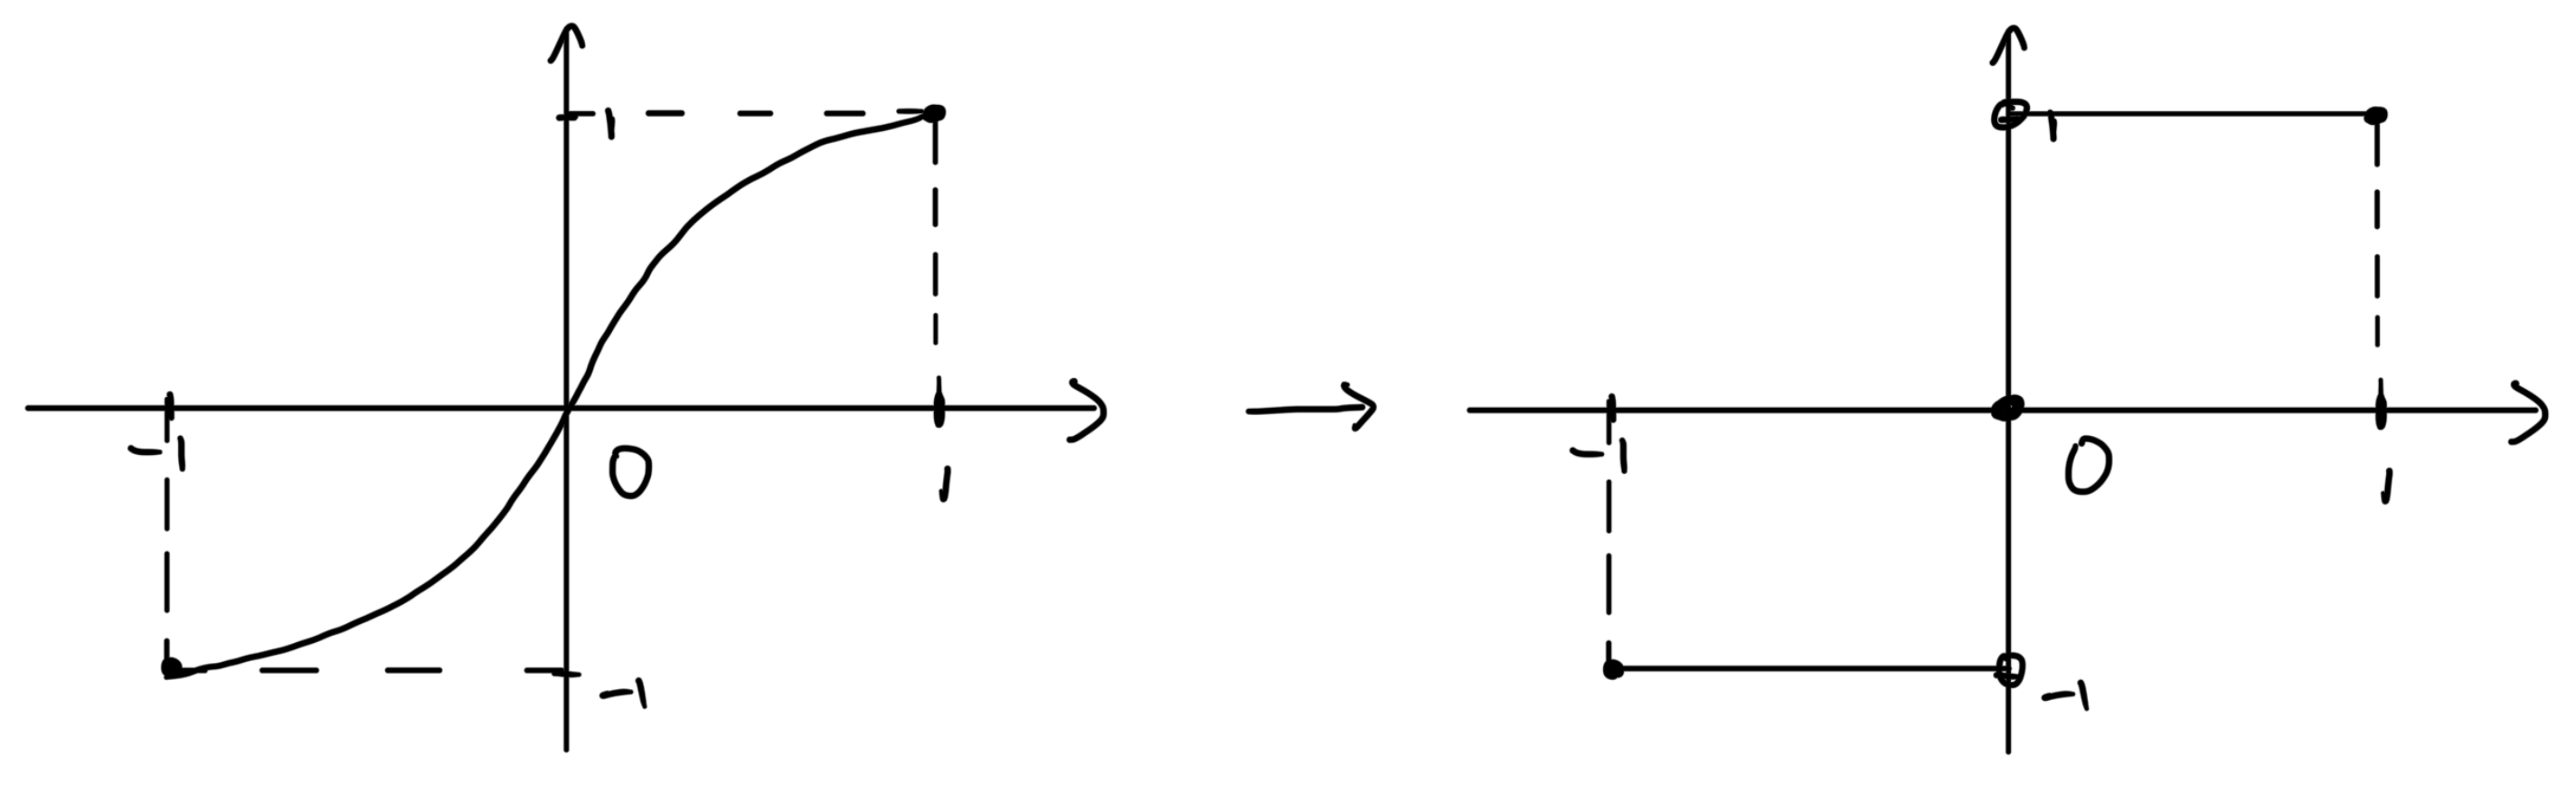
\includegraphics[width=0.9\linewidth]{fig/pointwise-limit.png}
    \caption{Pointwise Limit of the Sequence \(f_n\)}
    \label{fig:pointwise-limit}%
\end{figure}

\begin{example}[Pointwise Convergence does not Preserve Integrability]
    Let \(q_1, q_2, q_3, \ldots\) be an enumeration of \(\QQ \cap \ccintv{0}{1}\). Define \(\functiondomain{f_n}{\ccintv{0}{1}}{\RR}\) by
    \[
        f_n\pqty{x} = \begin{cases}
            1 & \qif x \in \Bqty{q_1, q_2, \ldots, q_n}, \\
            0 & \qif x \in \ccintv{0}{1} \setminus \Bqty{q_1, q_2, \ldots, q_n}.
        \end{cases}
    \]

    Note that \(f_n\) is integrable for all \(n \in \NN\), since it is continuous apart from points in \(\Bqty{q_1, q_2, \ldots. q_n}\).
    
    However, the pointwise limit of \(\pqty{f_n}\) is
    \[
        f\pqty{x} = \lim_{n \to \infty} f_n\pqty{x} = \indicator_{\QQ} \pqty{x}.
    \]
    which is not integrable.
\end{example}

A natural question that continues from integrability, is that if \(f_n\) is integrable for all \(n \in \NN\), does it follow that their pointwise limit \(f\), given integrable, integrates to the limit of the integrals?

\begin{figure}[ht!]
    \centering
    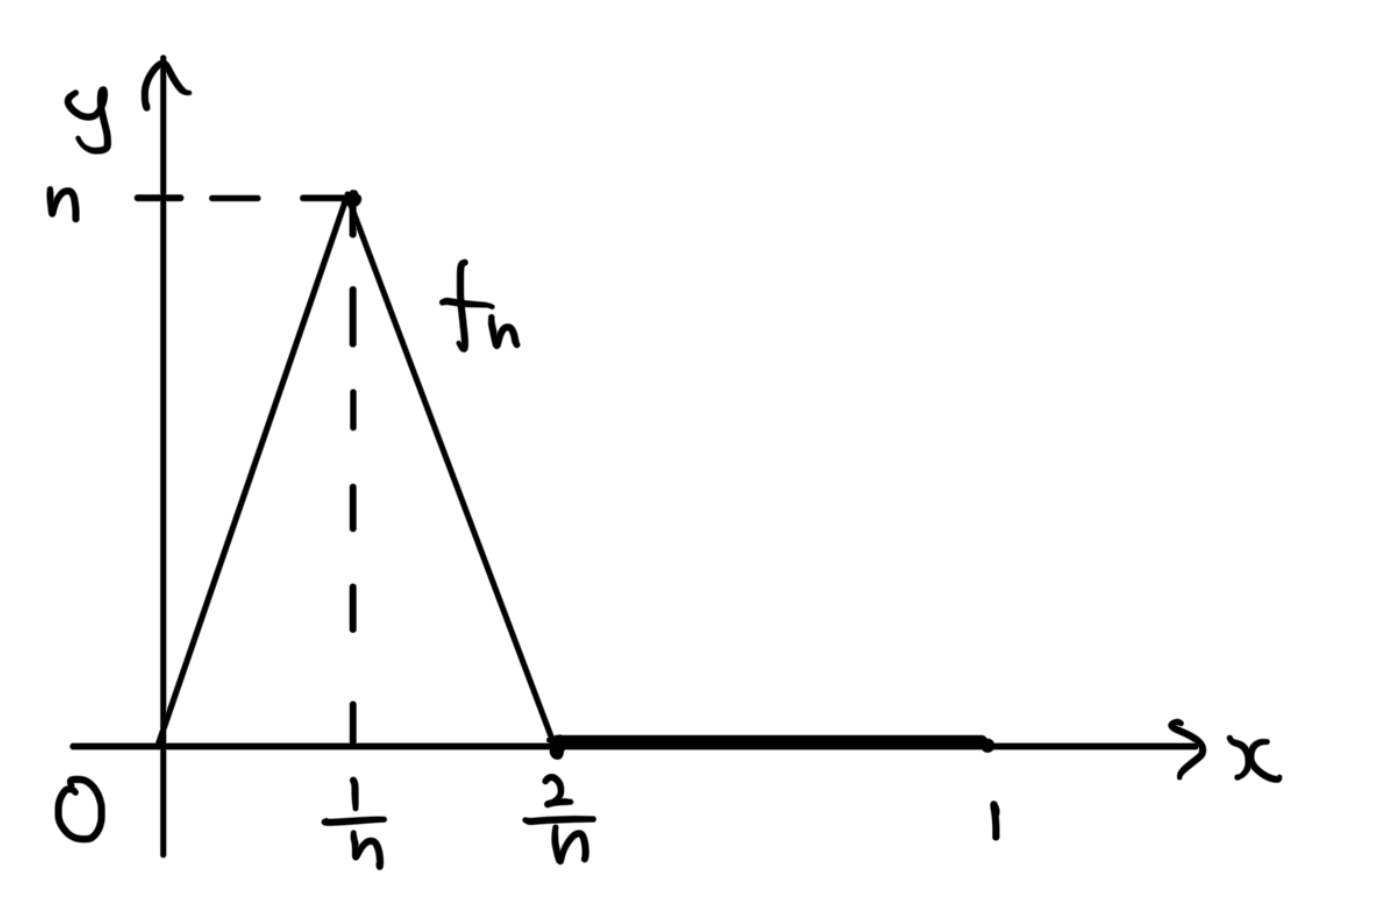
\includegraphics[width=0.7\linewidth]{fig/pointwise-limit-integral.png}
    \caption{Function in \autoref{ex:pointwise-limit-integral}}
    \label{fig:pointwise-limit-integral}%
\end{figure}

\begin{example}[Pointwise Limit does not Preserve Integral]
    \label{ex:pointwise-limit-integral}
    Consider the functions defined on \(\ccintv{0}{1}\) where
    \[
        f_n\pqty{x} = \begin{cases}
            n^2 x &\qif n \in \ccintv{0}{\flatfrac{1}{n}}, \\
            n^2 \pqty{\flatfrac{2}{n} - x} &\qif n \in \ccintv{\flatfrac{1}{n}}{\flatfrac{2}{n}}, \\
            0 &\qif x \in \ccintv{\flatfrac{2}{n}}{1}.
        \end{cases}
    \]

    Then clearly its pointwise limit is identically zero, since the triangle eventually moves to the left of any \(x\), however small (apart from \(x = 0\) which is identically zero), and hence
    \[
        \int_{0}^{1} f\pqty{x} \dd{x} = 0.
    \]

    However, notice that
    \[
        \int_{0}^{1} f_n\pqty{x} \dd{x} = 1, \quad \forall n \in \NN
    \]
    and hence
    \[
        \lim_{n \to \infty} \int_{0}^{1} f_n\pqty{x} \dd{x} = 1 \neq 0 = \int_{0}^{1} f\pqty{x} \dd{x} = \int_{0}^{1} \lim_{n \to \infty} f_n \pqty{x} \dd{x}
    \]
\end{example}

\subsection{Uniform Convergence}

We now give a stronger notion of convergence which preserves continuity and integrability. But clearly, we do not want too strong a notion of convergence, for example, the trivial one that \(f_n \to f\) means \(f = f_n\) for sufficiently large \(n\).

\begin{definition}[Uniform Convergence]
    Let \(\functiondomain{f_n, f}{E}{\RR}\) for \(n \in \NN\). We say that the sequence \(\pqty{f_n}\) \term{converges uniformly} to \(f\) on \(E\), if
    \[
        \forall \epsilon > 0, \exists N = N\pqty{\epsilon} \in \NN, \forall n \geq N, \forall x \in E: \abs{f_n\pqty{x} - f\pqty{x}} < \epsilon.
    \]

    This is equivalent to saying
    \[
        \forall \epsilon > 0, \exists N = N\pqty{\epsilon} \in \NN: n \geq N \implies \sup_{x \in E} \abs{f_n\pqty{x} - f\pqty{x}} < \epsilon,
    \]
    which in limit notation, reads
    \[
        \lim_{n \to \infty} \sup_{x \in E} \abs{f_n\pqty{x} - f\pqty{x}} = 0.
    \]

    We say \(f\) is the \term{uniform limit} of \(\pqty{f_n}\), and denote \(f_n \to f\) uniformly in \(E\).
\end{definition}

\begin{remark}
    Compare this with pointwise convergence, which states
    \[
        \forall x \in E, \forall \epsilon > 0, \exists N = N\pqty{\epsilon, x} \in \NN, \forall n \geq N: \abs{f_n\pqty{x} - f\pqty{x}} < \epsilon.
    \]

    Note that here, \(N\) may depend on \(x\). It is clear that uniform convergence implies pointwise convergence, while the converse is not true.
\end{remark}

\begin{example}[Pointwise Convergence does not imply Uniform Convergence]
    We look at the previous example, illustrated in \autoref{fig:pointwise-limit-integral}, where
        \[
            f_n\pqty{x} = \begin{cases}
                n^2 x &\qif n \in \ccintv{0}{\flatfrac{1}{n}}, \\
                n^2 \pqty{\flatfrac{2}{n} - x} &\qif n \in \ccintv{\flatfrac{1}{n}}{\flatfrac{2}{n}}, \\
                0 &\qif x \in \ccintv{\flatfrac{2}{n}}{1}.
            \end{cases}
        \]
        and \(f_n \to f\) where \(f\pqty{x} = 0\) \emph{pointwise} on \(\ccintv{0}{1}\). However, notice that
        \[
            \sup_{x \in \ccintv{0}{1}} \abs{f_n\pqty{x} - f\pqty{x}} = n \to \infty \neq 0,
        \]
        so \(f_n \notto f\) \emph{uniformly} on \(\ccintv{0}{1}\).
\end{example}

\begin{example}[Uniform Convergence depends on Domain]
    We look at the functions
    \[
        \function{f_n}{\RR}{\RR}{x}{\frac{x}{n}.}
    \]

    Then we have \(f_n \to 0\) \emph{pointwise} on \(\RR\), while
    \[
        \sup_{x \in \RR} \abs{f_n\pqty{x} - 0} = \infty,
    \]
    so \(f_n \notto 0\) \emph{uniformly} on \(\RR\).

    If we restrict the domain, we can achieve uniform convergence. Let \(a \in \oointv{0}{\plusinfty}\), \(\functiondomain{f_n}{\ccintv{-a}{a}}{\RR}\).

    Then
    \[
        \sup_{x \in \ccintv{-a}{a}} \abs{f_n\pqty{x}} = \sup_{x \in \ccintv{-a}{a}} \frac{\abs{x}}{n} = \frac{a}{n} \to 0,
    \]
    so \(f_n \to 0\) \emph{uniformly} on \(\ccintv{-a}{a}\).
\end{example}

Similarly to Cauchy sequences of real numbers, we can define a notion of Cauchy sequences of functions.

\subsection{Cauchy Criterion for Uniform Convergence}

\begin{definition}[Uniform Cauchy]
    Let \(\functiondomain{f_n}{E}{\RR}\) be a sequence of functions. We say \(\pqty{f_n}\) is \term{uniformly Cauchy} on \(E\), if
    \[
        \forall \epsilon > 0, \exists N = N\pqty{\epsilon} \in \NN: m, n \geq N \implies \sup_{x \in E} \abs{f_n\pqty{x} - f_m\pqty{x}} < \epsilon.
    \]
\end{definition}

\begin{theorem}[Cauchy Criterion for Uniform Convergence]
    \label{thm:cauchy-criterion-uniform-convergence}%
    Let \(\functiondomain{f_n}{E}{\RR}\) be a sequence of functions. Then \(\pqty{f_n}\) converges uniformly on \(E\) if and only if it is uniformly Cauchy on \(E\).
\end{theorem}

\begin{proof}
    Suppose \(\pqty{f_n}\) converges uniformly on \(E\) to some function \(f\). Let \(\epsilon > 0\), then there is some \(N = N\pqty{\epsilon} \in \NN\), such that for all \(n \geq N\)
    \[
        \sup_{x \in E} \abs{f_n\pqty{x} - f\pqty{x}} < \epsilon.
    \]

    Then for \(m, n \geq N\), we have
    \begin{align*}
        \abs{f_n\pqty{x} - f_m\pqty{x}} &\leq \abs{f_n\pqty{x} - f\pqty{x}} + \abs{f\pqty{x} - f_m\pqty{x}} \\
        &\leq \sup_{x \in E} \abs{f_n\pqty{x} - f\pqty{x}} + \sup_{x \in E} \abs{f\pqty{x} - f_m\pqty{x}},
    \end{align*}
    and hence
    \[
        \sup_{x \in E} \abs{f_n\pqty{x} - f_m\pqty{x}} \leq \sup_{x \in E} \abs{f_n\pqty{x} - f\pqty{x}} + \sup_{x \in E} \abs{f\pqty{x} - f_m\pqty{x}} < 2\epsilon.
    \]
    
    Now, suppose instead that \(\pqty{f_n}\) is uniformly Cauchy on \(E\). Then for all \(x \in E\), the sequence of real numbers \(\pqty{f_n \pqty{x}}\) is Cauchy. By Completeness of \(\RR\) (see \textit{IA Analysis I}), there exists a \emph{pointwise} limit \(f\pqty{x} = \lim_{n \to \infty} f_n\pqty{x}\) for all \(x \in E\). We now show that \(f_n \to f\) \emph{uniformly} on \(E\).

    To check that \(f_n \to f\) is uniform, let \(\epsilon > 0\). By hypothesis, there exists \(N\), such that for all \(m, n \geq N\), that
    \[
        \sup_{x \in E} \abs{f_n\pqty{x} - f_m\pqty{x}} < \epsilon.
    \]

    For a fixed \(x\), we have
    \begin{align*}
        \abs{f_n\pqty{x} - f\pqty{x}} &\leq \abs{f_n\pqty{x} - f_m\pqty{x}} + \abs{f_m\pqty{x} - f\pqty{x}} \\
        &< \epsilon + \abs{f_m\pqty{x} - f\pqty{x}} \\
        &< \epsilon + \epsilon = 2 \epsilon,
    \end{align*}
    if \(m\) is sufficiently large (since \(f_n \to f\) pointwise). Taking supremum over \(x \in E\), we have
    \[
        \sup_{x \in E} \abs{f_n\pqty{x} - f\pqty{x}} < 2 \epsilon,
    \]
    which shows that \(f_n \to f\) uniformly on \(E\).
\end{proof}

\begin{theorem}[Uniform Convergence preserves Continuity at a Point]
    Let \(\functiondomain{f_n, f}{\ccintv{a}{b}}{\RR}\) and \(f_n \to f\) uniformly. Suppose that, for some \(x_0 \in \ccintv{a}{b}\), \(f_n\) is continuous at \(x_0\) for all \(n\). Then \(f\) is continuous at \(x_0\).
\end{theorem}

\begin{proof}
    Let \(\epsilon > 0\). By uniform convergence, there is some \(N\), such that for all \(n \geq N\), we have
    \[
        \sup_{x \in \ccintv{a}{b}} \abs{f_n\pqty{x} - f\pqty{x}} < \epsilon.
    \]

    Then we have
    \begin{align*}
        \abs{f\pqty{y} - f\pqty{x}} &\leq \abs{f\pqty{y} - f_N\pqty{y}} + \abs{f_N\pqty{y} - f_N\pqty{x}} + \abs{f_N\pqty{x} - f\pqty{x}} \\
        &< 2\epsilon + \abs{f_N\pqty{y} - f_N\pqty{x}}.
    \end{align*}

    Take \(x = x_0\). If \(f_N\pqty{x}\) is continuous at \(x_0\), then for sufficiently small \(\delta = \delta\pqty{x_0, epsilon} > 0\), such that for all \(\abs{y - x_0 < \delta}\), we have
    \[
        \abs{f_N\pqty{y} - f_N\pqty{x_0}} < \epsilon,
    \]
    by continuity of \(f_N\) at \(x_0\). Hence, for all \(\abs{y - x_0} < \delta\), we have
    \[
        \abs{f\pqty{y} - f\pqty{x_0}} < 3 \epsilon,
    \]
    which shows that \(f\) is continuous at \(x_0\).
\end{proof}

Applying this to all \(x_0 \in \ccintv{a}{b}\) gives the following result.

\begin{corollary}[Uniform Convergence preserves Continuity]
    \label{cor:uniform-convergence-preserves-continuity}%
    Let \(\functiondomain{f_n, f}{\ccintv{a}{b}}{\RR}\) and \(f_n \to f\) uniformly. Suppose that, \(f_n\) is continuous on \(\ccintv{a}{b}\) for all \(n\). Then \(f\) is continuous on \(\ccintv{a}{b}\).
\end{corollary}

Recall from \textit{IA Analysis I} that \(\contClass{}\pqty{\ccintv{a}{b}}\) denotes the space of functions continuous on \(\ccintv{a}{b}\). Back in \textit{IA Analysis I}, recall that restricting to \(\QQ\) does \emph{not} preserve completeness of \(\RR\), since there are rational Cauchy sequences that do not converge in \(\QQ\). However, this space above is complete when we talk about uniform convergence (i.e. measuring `distance' using the supremum).

\begin{theorem}[Completeness of \(\contClass{}\pqty{\ccintv{a}{b}}\)]
    Let \(\pqty{f_n}\) be a uniformly Cauchy sequence in \(\contClass{}\pqty{\ccintv{a}{b}}\). Then there exists a continuous function \(f \in \contClass{}\pqty{\ccintv{a}{b}}\), such that \(f_n \to f\) uniformly on \(\ccintv{a}{b}\).
\end{theorem}

\begin{proof}
    By \autoref{thm:cauchy-criterion-uniform-convergence}, there exists a function \(f\) such that \(f_n \to f\) uniformly on \(\ccintv{a}{b}\). By \autoref{cor:uniform-convergence-preserves-continuity}, \(f\) is continuous on \(\ccintv{a}{b}\), so \(f \in \contClass{}\pqty{\ccintv{a}{b}}\).
\end{proof}